\documentclass{beamer}
\mode<presentation>
\usepackage{amsmath}
\usepackage{amssymb}
%\usepackage{advdate}
\usepackage{adjustbox}
\usepackage{subcaption}
\usepackage{enumitem}
\usepackage{multicol}
\usepackage{mathtools}
\usepackage{listings}
\usepackage{url}
\def\UrlBreaks{\do\/\do-}
\usetheme{Boadilla}
\usecolortheme{seahorse}
\setbeamertemplate{footline}
{
  \leavevmode%
  \hbox{%
  \begin{beamercolorbox}[wd=\paperwidth,ht=2.25ex,dp=1ex,right]{author in head/foot}%
    \insertframenumber{} / \inserttotalframenumber\hspace*{2ex} 
  \end{beamercolorbox}}%
  \vskip0pt%
}
\setbeamertemplate{navigation symbols}{}

\providecommand{\nCr}[2]{\,^{#1}C_{#2}} % nCr
\providecommand{\nPr}[2]{\,^{#1}P_{#2}} % nPr
\providecommand{\mbf}{\mathbf}
\providecommand{\pr}[1]{\ensuremath{\Pr\left(#1\right)}}
\providecommand{\qfunc}[1]{\ensuremath{Q\left(#1\right)}}
\providecommand{\sbrak}[1]{\ensuremath{{}\left[#1\right]}}
\providecommand{\lsbrak}[1]{\ensuremath{{}\left[#1\right.}}
\providecommand{\rsbrak}[1]{\ensuremath{{}\left.#1\right]}}
\providecommand{\brak}[1]{\ensuremath{\left(#1\right)}}
\providecommand{\lbrak}[1]{\ensuremath{\left(#1\right.}}
\providecommand{\rbrak}[1]{\ensuremath{\left.#1\right)}}
\providecommand{\cbrak}[1]{\ensuremath{\left\{#1\right\}}}
\providecommand{\lcbrak}[1]{\ensuremath{\left\{#1\right.}}
\providecommand{\rcbrak}[1]{\ensuremath{\left.#1\right\}}}
\theoremstyle{remark}
\newtheorem{rem}{Remark}
\newcommand{\sgn}{\mathop{\mathrm{sgn}}}
\providecommand{\abs}[1]{\left\vert#1\right\vert}
\providecommand{\res}[1]{\Res\displaylimits_{#1}} 
\providecommand{\norm}[1]{\lVert#1\rVert}
\providecommand{\mtx}[1]{\mathbf{#1}}
\providecommand{\mean}[1]{E\left[ #1 \right]}
\providecommand{\fourier}{\overset{\mathcal{F}}{ \rightleftharpoons}}
%\providecommand{\hilbert}{\overset{\mathcal{H}}{ \rightleftharpoons}}
\providecommand{\system}{\overset{\mathcal{H}}{ \longleftrightarrow}}
	%\newcommand{\solution}[2]{\textbf{Solution:}{#1}}
%\newcommand{\solution}{\noindent \textbf{Solution: }}
\providecommand{\dec}[2]{\ensuremath{\overset{#1}{\underset{#2}{\gtrless}}}}
\newcommand{\myvec}[1]{\ensuremath{\begin{pmatrix}#1\end{pmatrix}}}
\let\vec\mathbf

\lstset{
%language=C,
frame=single, 
breaklines=true,
columns=fullflexible
}

\numberwithin{equation}{section}

\title{Mat Geo Presentation}
\author{CHARAN RONGALI \\ Electrical Engineering,\\IIT Hyderabad.}

\date{\today} 
\begin{document}

\begin{frame}
\titlepage
\end{frame}

\section*{Outline}
\begin{frame}
\tableofcontents
\end{frame}
\section{Problem}
\begin{frame}
\frametitle{Problem Statement}
Find the area of the region in the first quadrant enclosed by $x$-axis, line $y=x$ and the circle $x^2 + y^2 = 32$.

\end{frame}

%\subsection{Literature}
\section{Solution}
\subsection{Matrix Equation}
\begin{frame}
\frametitle{Matrix Equation}
\begin{align}
\label{eq:equation}
g(x) &= \vec{x}^\top \vec{V}\vec{x}+2\vec{u}^\top \vec{x}+f=0
\end{align}
%\begin{enumerate}[label=(\roman*)]
\begin{align}
\begin{split}
\vec{V} &= \myvec{1 & 0
                 \\
		 0 & 1}\\
	\vec{u} &= \vec{0} \\
	f &= -32\\
\end{split}
\end{align}
\begin{align}
Line: \vec{x} &= \vec{h}+k\vec{m} 
\end{align}
\begin{align}
	\vec{h} &= \myvec{0 \\ 0} \\
	\vec{m} &= \myvec{\frac{1}{\sqrt{2}} \\ \frac{1}{\sqrt{2}}}
\end{align}
\begin{align}
\label{eq:points}
	\vec{x_i} &= \vec{h}+k_{i}\vec{m}
\end{align}
\end{frame}
\subsection{Point of Intersection}
\begin{frame}
\frametitle{Point of Intersection}
	By Substituting \eqref{eq:points} in \eqref{eq:equation} we get two values of $k_1$ and $k_2$
%
\begin{align}
	k_1 &= \frac{1}{\vec{m}^\top \vec{V}\vec{m}}\brak{-m^\top\brak{\vec{V}\vec{h}+\vec{u}}+ \sqrt{[\vec{m}^\top \brak{\vec{V}\vec{h}+\vec{u}}]^2 - g(\vec{h})\brak{\vec{m}^\top\vec{V}\vec{m}}}}  \\
	k_2 &= \frac{1}{\vec{m}^\top \vec{V}\vec{m}}\brak{-m^\top\brak{\vec{V}\vec{h}+\vec{u}}- \sqrt{[\vec{m}^\top \brak{\vec{V}\vec{h}+\vec{u}}]^2 - g(\vec{h})\brak{\vec{m}^\top\vec{V}\vec{m}}}}
\end{align}
so we get 
\begin{align}
	k_i &= \pm 4\sqrt{2}\\
    x_i &= \pm \myvec{4\\4}
\end{align}
As we are only considering the first quadrant, we take the point of intersection as $\myvec{4\\4}$.

\end{frame}
%\section{Plot}
\subsection{Area}
\begin{frame}[fragile]
\frametitle{Area}
\begin{align}
	Area: A &= A_1 + A_2 \label{eq:total_area} \\
    A_1 &= \int_{0}^{4} x \, dx \\
    &= \sbrak{\frac{x^2}{2}}_{0}^{4} \\
    &= 8 \\
    A_2 &= \int_{4}^{4\sqrt{2}} \sqrt{32 - x^2} \, dx \\
    &= \sbrak{\frac{x\sqrt{32 - x^2}}{2} + 16\sin^{-1}{\frac{x}{4\sqrt{2}}}}_{4}^{4\sqrt{2}} \\
    &= 4\pi - 8 \\
    \therefore A &= A_1 + A_2 = 4\pi \approx 12.56637
\end{align}%
\end{frame}
\subsection{computational solutions}
\begin{frame}
\frametitle{computational solutions}

Area Approximation can be done by various methods:\\
	1) Left Riemann sum\\
	2) Right Riemann sum\\
	3) Mid Point Rule\\
	4) Trapezoidal Rule\\
	5) Simpson's Rule\\
	6) Method of Exhaustion

\end{frame}
\subsection{Left Riemann}
\begin{frame}
\frametitle{Left Riemann}
The Left Riemann Sum approximates the area by using rectangles whose heights are determined by the left endpoint of each subinterval. Let \(h\) be the step size, and \(A_n\) be the area till \(x_n\), then:
\begin{align}
    A_n &= h\sum_{i=0}^{n-1} y(x_i),\\
    A_{n+1} &= A_n + h y(x_n).
\end{align}
\frametitle{\hspace{0.5em} Left Riemann \hfill 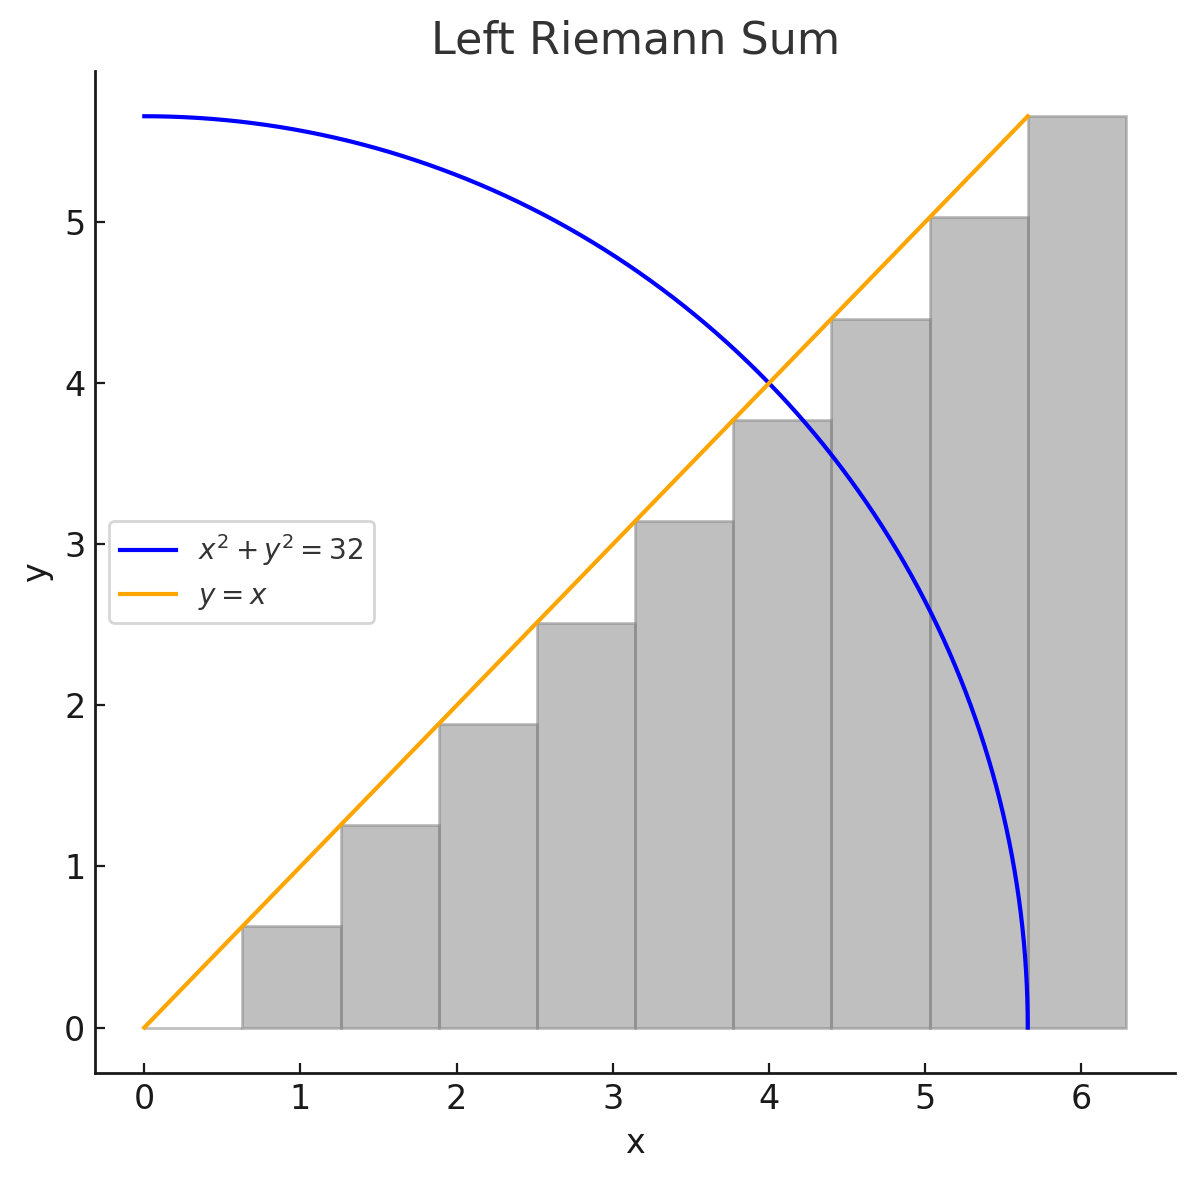
\includegraphics[scale=0.1]{figs/1.png}}

\end{frame}
\subsection{Right Riemann}
\begin{frame}
\frametitle{Right Riemann}
The Right Riemann Sum approximates the area by using rectangles whose heights are determined by the right endpoint of each subinterval. Let \(h\) be the step size, and \(A_n\) be the area till \(x_n\), then:
\begin{align}
    A_n &= h\sum_{i=1}^n y(x_i),\\
    A_{n+1} &= A_n + h y(x_{n+1}).
\end{align}
\frametitle{\hspace{0.5em} Right Riemann \hfill 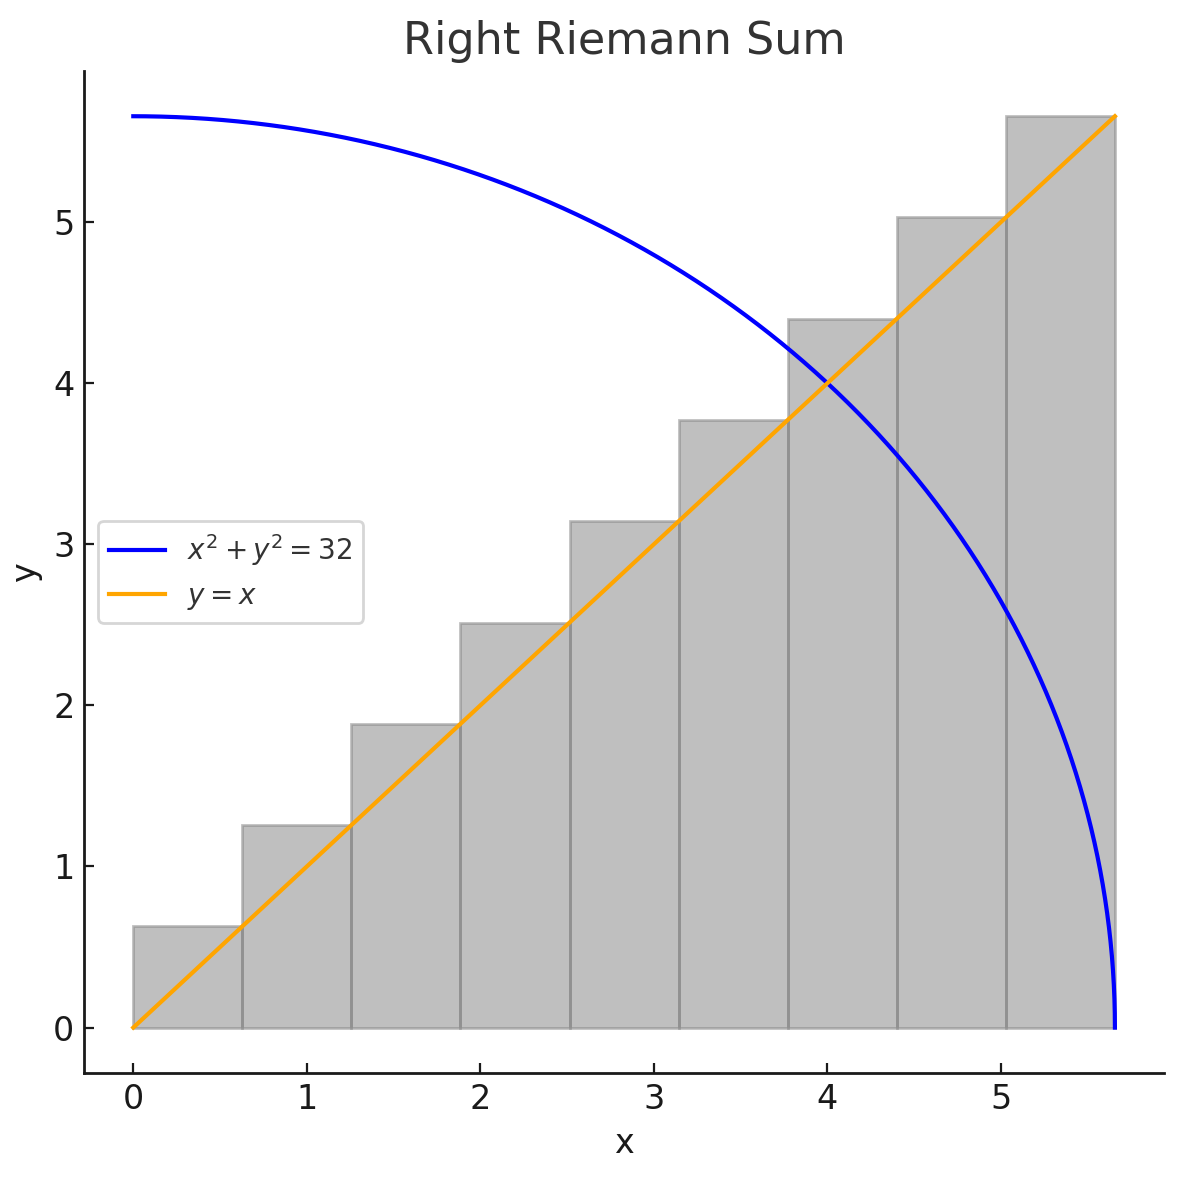
\includegraphics[scale=0.1]{figs/2.png}}

\end{frame}
\subsection{Mid Point Rule}
\begin{frame}
\frametitle{Mid Point Rule}
The Midpoint Rule approximates the area by using rectangles whose heights are determined by the midpoint of each subinterval. Let \(h\) be the step size, and \(A_n\) be the area till \(x_n\), then:
\begin{align}
    A_n &= h\sum_{i=1}^n y\left(x_{i - \frac{1}{2}}\right), \quad x_{i - \frac{1}{2}} = x_{i-1} + \frac{h}{2},\\
    A_{n + 1} &= A_n + h\cdot y\left(x_n + \frac{h}{2}\right).
\end{align}
\frametitle{\hspace{0.5em} Mid Point Rule \hfill 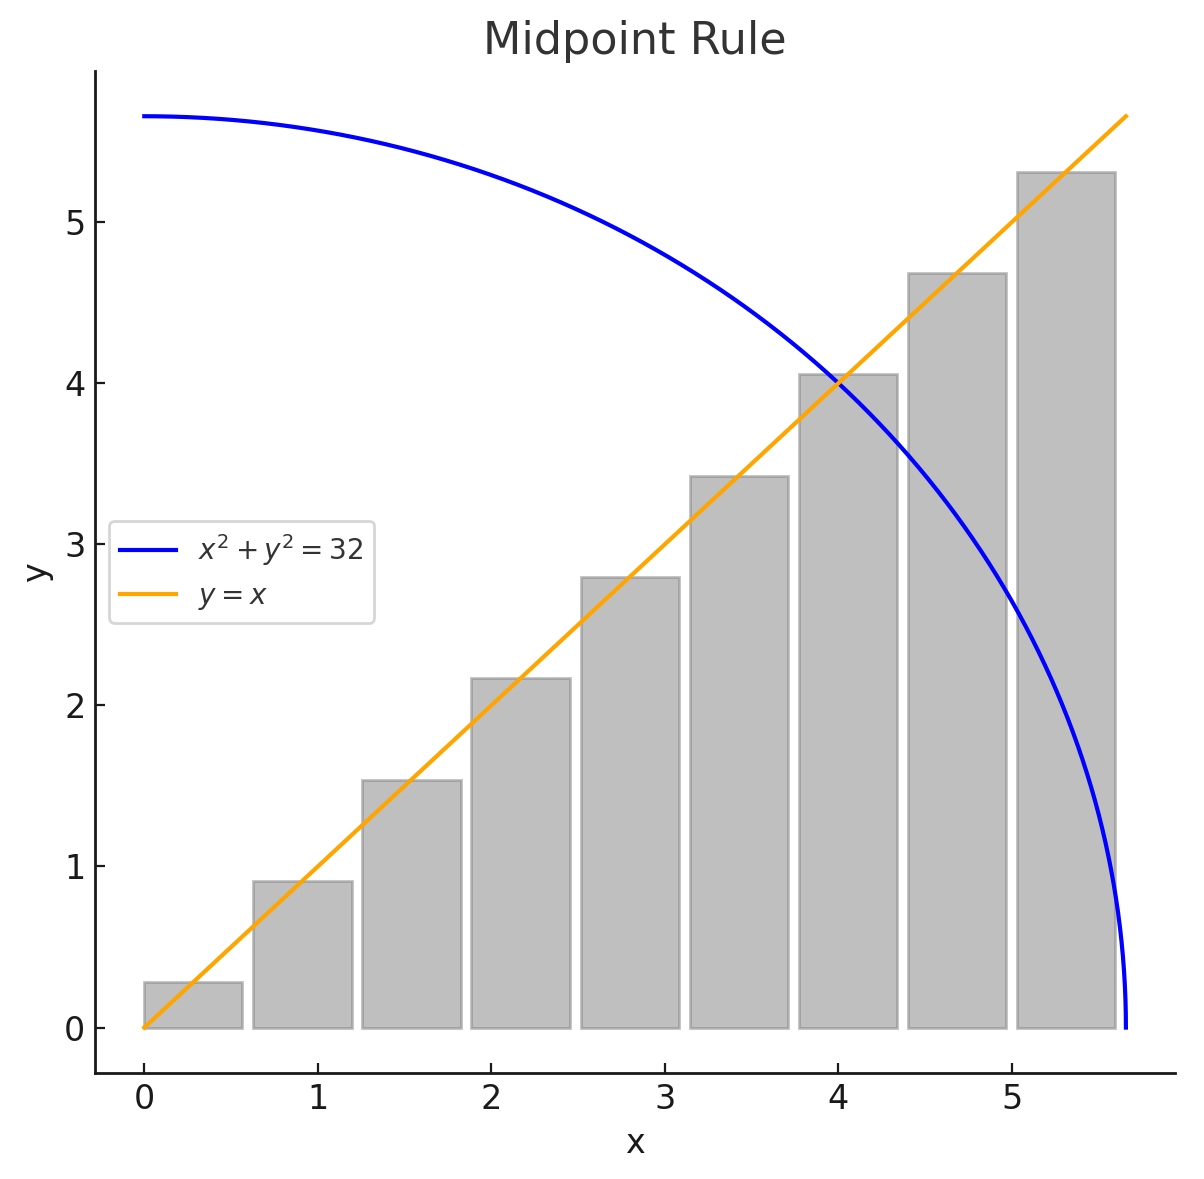
\includegraphics[scale=0.1]{figs/3.png}}

\end{frame}
\subsection{Method of Exhaustion}
\begin{frame}
\frametitle{Method of Exhaustion}
This method divides the area into smaller shapes \((\text{rectangles, trapeziums, etc.})\) and calculates the total area as the limit of the sum as \(n \to \infty\). The area \(A_n\) is given by:
\begin{align}
    A_n &= \sum_{i=1}^n A_i, \quad \text{where } A_i \text{ is the area of each small shape.}
\end{align}
\frametitle{\hspace{0.5em} Method of Exhaustion \hfill 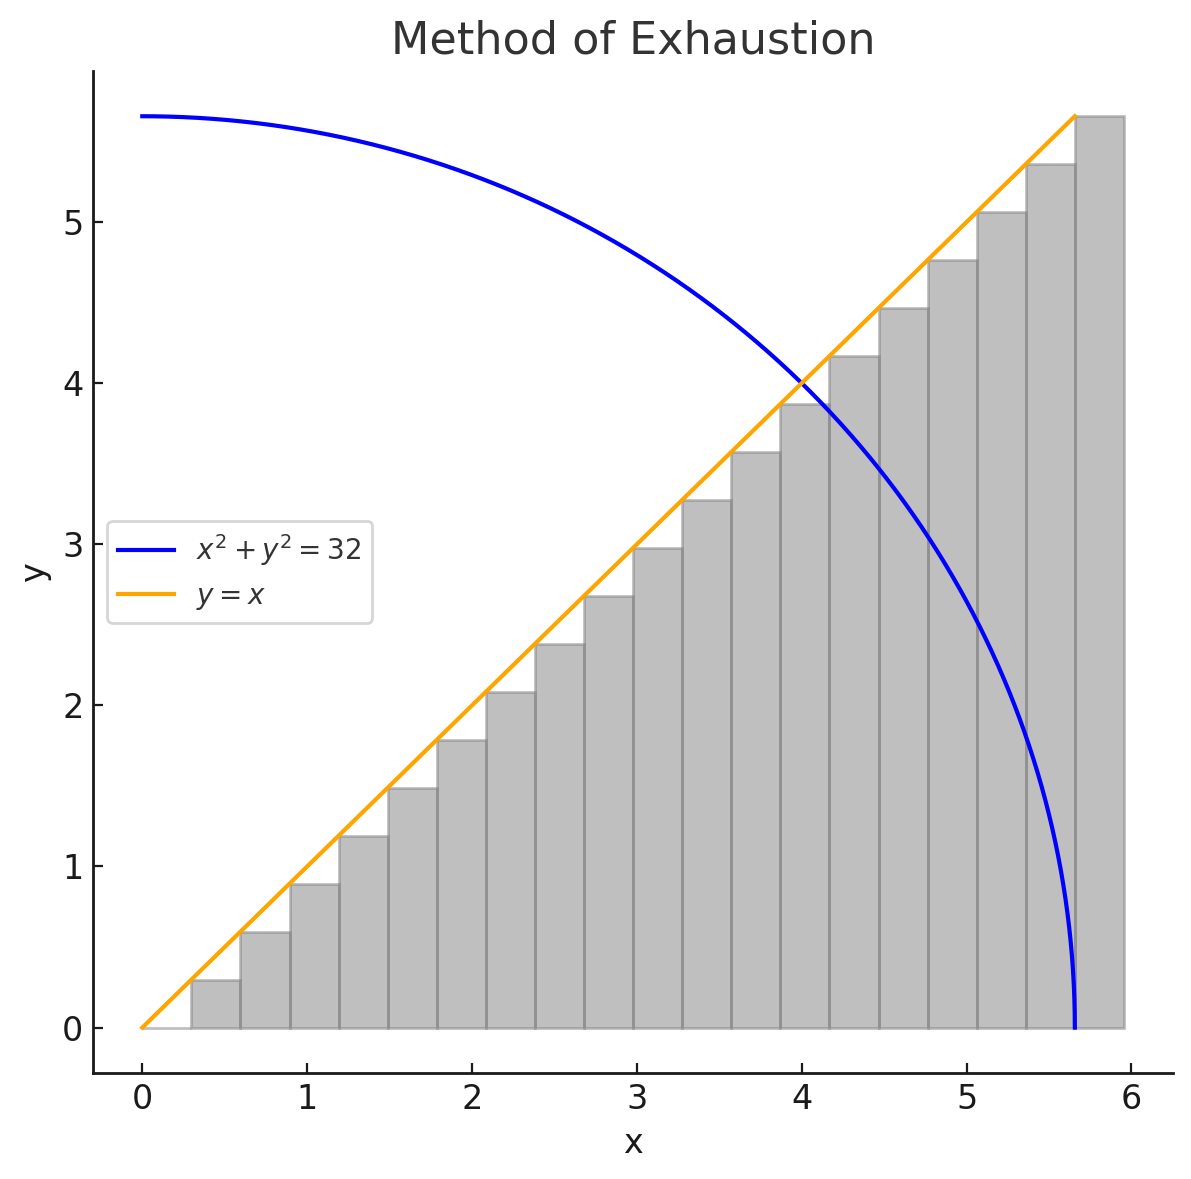
\includegraphics[scale=0.1]{figs/6.png}}
\end{frame}
\begin{frame}
For rectangles:
\begin{align}
    A_i &= h \cdot y(x_i), \quad \text{where } h \to 0,\\
    A_{n+1} &= A_n + h y(x_n).
\end{align}
For trapeziums:
\begin{align}
    A_i &= \frac{h}{2}\left(y(x_{i-1}) + y(x_i)\right),\\
    A_{n+1} &= A_n + \frac{h}{2}\left(y(x_n) + y(x_n + h)\right).
\end{align}
\end{frame}
\subsection{Trapezoidal Rule}
\begin{frame}
\frametitle{Trapezoidal Rule}
\newline
In the Trapezoidal method, We split the area into multiple small trapeziums \brak{\text{like small strips}}, and we sum up all the trapezium areas to find the total area. 
\newline
We discretize the range of $x$-coordinates with uniform step-size $h \to 0$, such that the discretized points are $x_0$, $x_1$, $\dots$, $x_n$ and $x_{n + 1} = x_n + h$.
\newline
Let the sum of trapizoidal areas till $x_n$ be $A_n$ and $y = y\brak{x}$, then we write the $\textbf{difference equation}$,
\begin{align}
    A_n &= \frac{h}{2}\brak{y\brak{x_0} + y\brak{x_1}} + \frac{h}{2}\brak{y\brak{x_1} + y\brak{x_2}} + \dots + \frac{h}{2}\brak{y\brak{x_{n - 1}} + y\brak{x_{n}}}\\
    A_n &= h\brak{\frac{y\brak{x_0}}{2} + y\brak{x_1} + y\brak{x_2} \dots \frac{y\brak{x_n}}{2}}\\
    A_{n + 1} &= A_n + \frac{h}{2}\brak{y\brak{x_{n + 1}} + y\brak{x_n}} \text{, } x_{n + 1} = x_n + h\\
    A_{n + 1} &= A_n + \frac{h}{2}\brak{y\brak{x_n + h} + y\brak{x_n}}
\end{align}
\end{frame}
\begin{frame}
By the first principle of derivative,
\begin{align}
    y^{\prime}\brak{x} &= \lim_{h\to0} \frac{y\brak{x + h} - y\brak{x}}{h}\\
    y\brak{x + h} &= y\brak{x} + h\brak{y^{\prime}\brak{x}} \text{, } h\to0
\end{align}
Rewriting the difference equation, we get,
\begin{align}
    A_{n + 1} &= A_n + \frac{h}{2}\brak{y\brak{x_n} + hy^{\prime}\brak{x_n} + y\brak{x_n}}\\
    A_{n + 1} &= A_n + h\brak{y\brak{x_n} + \frac{h}{2}y^{\prime}\brak{x_n}}\\
    A_{n + 1} &= A_n + hy\brak{x_n} + \frac{h^2}{2}y^{\prime}\brak{x_n}
\end{align}
For the given area enclosed, we take
\begin{align}
    y\brak{x} =
    \begin{cases}
        x & \quad 0 < x < 4\\
	    \sqrt{32 - x^2} & \quad 4 < x < 4\sqrt{2}
    \end{cases}
\end{align}
\end{frame}
\begin{frame}

\frametitle{\hspace{0.5em} Trapezoidal Rule \hfill 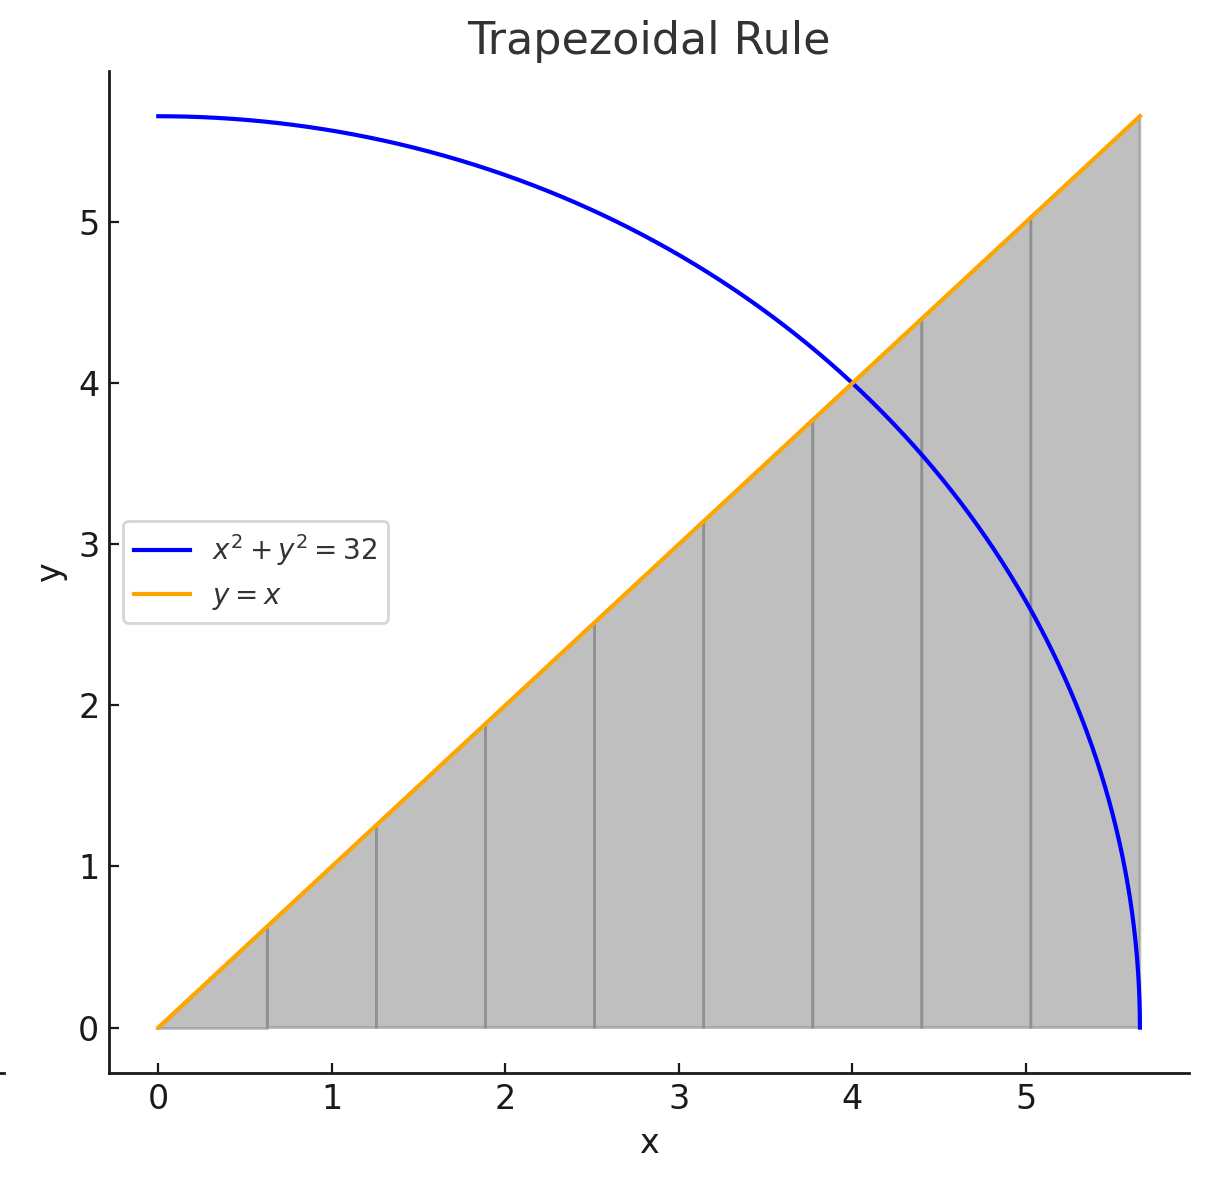
\includegraphics[scale=0.1]{figs/4.png}}
Substituting $y\brak{x}$, the equation becomes,
\begin{align}
    A_{n + 1} &=
    \begin{cases}
        A_n + h x_n + \frac{h^2}{2} & \quad 0 < x_n < 4\\
	    A_n + h\sqrt{32 - x_n^2} + \frac{h^2}{2}\brak{\frac{-x_n}{32 - x_n^2}} & \quad 4 < x_n < 4\sqrt{2}
    \end{cases}\\
    x_{n + 1} &= x_n + 1
\end{align}
Computational Area: 12.56576
\newline
Theoritical Area: 12.56637
\newline
Plotting the given equations, we get the following plot.

\end{frame}


\subsection{Plot}
\begin{frame}
\frametitle{Plot}
\begin{figure}[h]
\centering
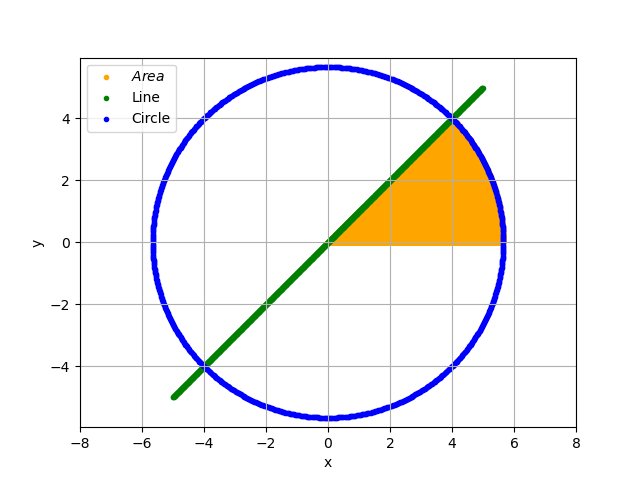
\includegraphics[scale=0.7]{figs/graph.png}
\label{Fig}
\end{figure}

\end{frame}
\end{document}
